\documentclass{icnmmf5}
\selectlanguage{english}
\usepackage{natbib}
\bibliographystyle{abbrv}

% Your title goes here.
\title{Prediction of averaged inter particles' properties within a buoyant emulsion by the use of \textit{Nearest Particle Statistics}}

% The author list. A \thanks{} is used to give an email address.
% This is only required for the corresponding author.
\author{Fintzi Nicolas\thanks{Email:~nicolas.fintzi@ifpen.fr}\\IFP Energies Nouvelles\and
Pierson Jean-Lou\thanks{Email:~jean-lou.pierson@ifpen.fr}\\IFP Energies Nouvelles
\and
Stéphane Popinet\thanks{Email:~popinet@basilisk.fr}\\Sorbonne Universite}

% Empty date for \maketitle. Don't modify.
\date{}

\begin{document}
\maketitle

The population balance and averaged Navier Stokes equations have been used in engineering for decades. 
However, there is a clear lack of accurate closure regarding the coalescence source term in emulsion modeling.  
Therefore, in a multiscale strategy 
We used the code Basilisk ({http://basilisk.fr}) to perform tri-periodic simulations of buoyant emulsions, see Figure \ref{fig:tower}~(left). 
In addition, to providing data for the closure terms appearing in the averaged models (PBE and averaged Navier-Stokes equations), tri-periodic simulations are of great interest to understand and describe pairwise interactions of rising droplets. Witch is crucial information, if we wish to model coalescence phenomenon based on film drainage analysis. 

Therefore, in this work, we present a statistical analysis based on the recent Nearest Particle Statistics framework of \cite{zhang2021ensemble}.
We define a pair by a particle and its nearest neighbor. 
This enables us to get the averaged relative or absolute characteristics of droplets pairs during collisions.
% , and thus deduce the nature of the average interaction. 
From this analysis we are able to propose a qualitative description of :
the relative position of particles, the relative kinematic and dynamical behavior of colliding pairs (see Figure \ref{fig:tower}~(middle)), the wake of a non-isolated particle (see Figure \ref{fig:tower}~(middle)).
From the observation of these statistics we can clearly identify drafting kissing thumbing mechanism, clustering phenomenon and the different wake produce by the droplets.   
We also provide quantitative results such as the
% mean time of interaction and the mean kinematic energy loss during an interaction. 
the particle-fuild-particle stress tensor, such as it is defined in \cite{zhang2021ensemble} (see \ref{fig:tower}~(right)). 
This tensor describes long range interaction between droplets through the fluid and has been shown to be crucial to ensure the hyperbolicity of the averaged NS equations \cite{fox2022hyperbolic}. 

Overall, we provide an intuitive understanding of pairwise interactions between particles, but also between the ambient fluid and the particles. 




% rigorous formulation for the mean time of interaction between droplets, the dyna

% Additionally, we sample eulerian fields such as fluid velocity and pressure, conditional on the presence of the nearest neighboring particle. 
% This enables us to reconstruct, what we call the undisturbed disturbance velocity of a droplet within a non-dilute emulsion. 
% From the shape of the 


\begin{figure}[b]
  \begin{center}
   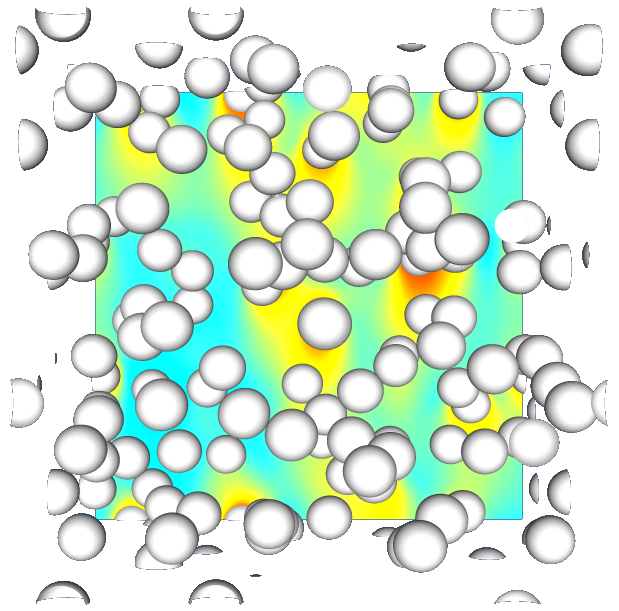
\includegraphics[height=4.5cm]{image/3D/P_PHI_5.png}
   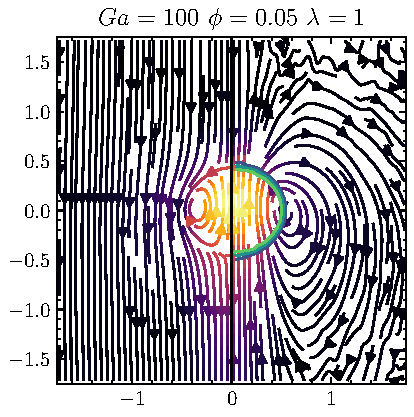
\includegraphics[height=4.5cm]{image/HOMOGENEOUS/Stream/Stream_PHI_5_Ga_100_l_1.pdf}
   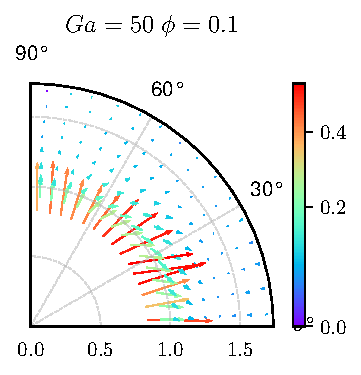
\includegraphics[height=4.5cm]{image/HOMOGENEOUS/fDrop/F_mu_r_1_0_Ga_50_PHI_0_1.pdf}
  \end{center}
  \caption{(left) DNS of a buoyant emulsion with finite size 125 droplets.
  (middle) Reconstruction of the nearest particle averaged eulerian velocity field.
  (right) Reconstruction of the nearest particle averaged particle center of mass acceleration field.}
  \label{fig:tower}
\end{figure}

% \LaTeX\ users can modify the source file of this document to create their abstract. %Similarly, the
%Microsoft Word document can be used. 
% Formatting the title and authors should be clear from these examples. 
% An email address is only required for the corresponding author. 
% The full document should not contain sections and should not exceed one A4 pages.
% Please include tables and figures like Fig.~\ref{fig:tower} at the end of the paper.
% The bibliography should be formatted as indicated below in this template, references should be
% ordered as they appear in the text like \cite{book1, article1, conf1}.


%\section*{Submission}
%
%For the initial submission the authors may submit either source files of the document or a PDF
%file. \LaTeX\ users should not forget to add separate files like figures to their \LaTeX\ files.
%For the final submission of accepted (and possibly revised) abstracts only the source files can be
%submitted, i.e.\ for \LaTeX\ users the \verb+*.tex+ document and possibly \verb+*.eps+ figures or
%for Microsoft Word users the \verb+*.doc+ or \verb+*.docx+ file.
%
%\section*{Acknowledgements}
%
%The style for this template has been created by combining several guidelines found on the internet.
%The picture in Fig.~\ref{fig:tower} is from Wikipedia.
\bibliography{Bib/bib_bulles.bib}

% \begin{thebibliography}{9}
% \bibitem{book1}
% A. Lastname, \textit{Book title}, 2$^{\rm nd}$ edition, Publisher, City, 2017.

% \bibitem{article1}
% A. Lastname1, B. Lastname2, \textit{Paper title}, Journal name, \textbf{11}(1), pp.\ 101--109,
% 2017.

% \bibitem{conf1}
% Lastname1, A., Lastname2, B., \emph{Paper title}, pp.\ 201--202 in Proceedings of the EUROMECH
% Colloquium 596, Venice, Italy, 2018.

% \end{thebibliography}

\end{document}
%%%%%%%%%%%%%%%%%%%%%%%%%%%%%%%%%%%%%%%%%%%%%%%%%%%%%%%%%%%%%%%%%%%%%%%%%%%%%%%%%%%%%%%%%%%%%%%%%%%%%%%
